% Options for packages loaded elsewhere
\PassOptionsToPackage{unicode}{hyperref}
\PassOptionsToPackage{hyphens}{url}
\documentclass[
  french,
]{article}
\usepackage{xcolor}
\usepackage[margin=2cm]{geometry}
\usepackage{amsmath,amssymb}
\setcounter{secnumdepth}{-\maxdimen} % remove section numbering
\usepackage{iftex}
\ifPDFTeX
  \usepackage[T1]{fontenc}
  \usepackage[utf8]{inputenc}
  \usepackage{textcomp} % provide euro and other symbols
\else % if luatex or xetex
  \usepackage{unicode-math} % this also loads fontspec
  \defaultfontfeatures{Scale=MatchLowercase}
  \defaultfontfeatures[\rmfamily]{Ligatures=TeX,Scale=1}
\fi
\usepackage{lmodern}
\ifPDFTeX\else
  % xetex/luatex font selection
\fi
% Use upquote if available, for straight quotes in verbatim environments
\IfFileExists{upquote.sty}{\usepackage{upquote}}{}
\IfFileExists{microtype.sty}{% use microtype if available
  \usepackage[]{microtype}
  \UseMicrotypeSet[protrusion]{basicmath} % disable protrusion for tt fonts
}{}
\makeatletter
\@ifundefined{KOMAClassName}{% if non-KOMA class
  \IfFileExists{parskip.sty}{%
    \usepackage{parskip}
  }{% else
    \setlength{\parindent}{0pt}
    \setlength{\parskip}{6pt plus 2pt minus 1pt}}
}{% if KOMA class
  \KOMAoptions{parskip=half}}
\makeatother
\usepackage{color}
\usepackage{fancyvrb}
\newcommand{\VerbBar}{|}
\newcommand{\VERB}{\Verb[commandchars=\\\{\}]}
\DefineVerbatimEnvironment{Highlighting}{Verbatim}{commandchars=\\\{\}}
% Add ',fontsize=\small' for more characters per line
\newenvironment{Shaded}{}{}
\newcommand{\AlertTok}[1]{\textcolor[rgb]{1.00,0.00,0.00}{\textbf{#1}}}
\newcommand{\AnnotationTok}[1]{\textcolor[rgb]{0.38,0.63,0.69}{\textbf{\textit{#1}}}}
\newcommand{\AttributeTok}[1]{\textcolor[rgb]{0.49,0.56,0.16}{#1}}
\newcommand{\BaseNTok}[1]{\textcolor[rgb]{0.25,0.63,0.44}{#1}}
\newcommand{\BuiltInTok}[1]{\textcolor[rgb]{0.00,0.50,0.00}{#1}}
\newcommand{\CharTok}[1]{\textcolor[rgb]{0.25,0.44,0.63}{#1}}
\newcommand{\CommentTok}[1]{\textcolor[rgb]{0.38,0.63,0.69}{\textit{#1}}}
\newcommand{\CommentVarTok}[1]{\textcolor[rgb]{0.38,0.63,0.69}{\textbf{\textit{#1}}}}
\newcommand{\ConstantTok}[1]{\textcolor[rgb]{0.53,0.00,0.00}{#1}}
\newcommand{\ControlFlowTok}[1]{\textcolor[rgb]{0.00,0.44,0.13}{\textbf{#1}}}
\newcommand{\DataTypeTok}[1]{\textcolor[rgb]{0.56,0.13,0.00}{#1}}
\newcommand{\DecValTok}[1]{\textcolor[rgb]{0.25,0.63,0.44}{#1}}
\newcommand{\DocumentationTok}[1]{\textcolor[rgb]{0.73,0.13,0.13}{\textit{#1}}}
\newcommand{\ErrorTok}[1]{\textcolor[rgb]{1.00,0.00,0.00}{\textbf{#1}}}
\newcommand{\ExtensionTok}[1]{#1}
\newcommand{\FloatTok}[1]{\textcolor[rgb]{0.25,0.63,0.44}{#1}}
\newcommand{\FunctionTok}[1]{\textcolor[rgb]{0.02,0.16,0.49}{#1}}
\newcommand{\ImportTok}[1]{\textcolor[rgb]{0.00,0.50,0.00}{\textbf{#1}}}
\newcommand{\InformationTok}[1]{\textcolor[rgb]{0.38,0.63,0.69}{\textbf{\textit{#1}}}}
\newcommand{\KeywordTok}[1]{\textcolor[rgb]{0.00,0.44,0.13}{\textbf{#1}}}
\newcommand{\NormalTok}[1]{#1}
\newcommand{\OperatorTok}[1]{\textcolor[rgb]{0.40,0.40,0.40}{#1}}
\newcommand{\OtherTok}[1]{\textcolor[rgb]{0.00,0.44,0.13}{#1}}
\newcommand{\PreprocessorTok}[1]{\textcolor[rgb]{0.74,0.48,0.00}{#1}}
\newcommand{\RegionMarkerTok}[1]{#1}
\newcommand{\SpecialCharTok}[1]{\textcolor[rgb]{0.25,0.44,0.63}{#1}}
\newcommand{\SpecialStringTok}[1]{\textcolor[rgb]{0.73,0.40,0.53}{#1}}
\newcommand{\StringTok}[1]{\textcolor[rgb]{0.25,0.44,0.63}{#1}}
\newcommand{\VariableTok}[1]{\textcolor[rgb]{0.10,0.09,0.49}{#1}}
\newcommand{\VerbatimStringTok}[1]{\textcolor[rgb]{0.25,0.44,0.63}{#1}}
\newcommand{\WarningTok}[1]{\textcolor[rgb]{0.38,0.63,0.69}{\textbf{\textit{#1}}}}
\usepackage{longtable,booktabs,array}
\usepackage{caption}
\captionsetup[table]{skip=6pt}
\newcounter{none} % for unnumbered tables
\usepackage{calc} % for calculating minipage widths
% Correct order of tables after \paragraph or \subparagraph
\usepackage{etoolbox}
\makeatletter
\patchcmd\longtable{\par}{\if@noskipsec\mbox{}\fi\par}{}{}
\makeatother
\usepackage{graphicx}
\makeatletter
\newsavebox\pandoc@box
\newcommand*\pandocbounded[1]{% scales image to fit in text height/width
  \sbox\pandoc@box{#1}%
  \Gscale@div\@tempa{\textheight}{\dimexpr\ht\pandoc@box+\dp\pandoc@box\relax}%
  \Gscale@div\@tempb{\linewidth}{\wd\pandoc@box}%
  \ifdim\@tempb\p@<\@tempa\p@\let\@tempa\@tempb\fi% select the smaller of both
  \ifdim\@tempa\p@<\p@\scalebox{\@tempa}{\usebox\pandoc@box}%
  \else\usebox{\pandoc@box}%
  \fi%
}
% Set default figure placement to htbp
\def\fps@figure{htbp}
\makeatother
\usepackage{svg}
\ifLuaTeX
\usepackage[bidi=basic,shorthands=off]{babel}
\else
\usepackage[bidi=default,shorthands=off]{babel}
\fi
\ifLuaTeX
  \usepackage{selnolig} % disable illegal ligatures
\fi
\setlength{\emergencystretch}{3em} % prevent overfull lines
\providecommand{\tightlist}{%
  \setlength{\itemsep}{0pt}\setlength{\parskip}{0pt}}
\usepackage{bookmark}
\IfFileExists{xurl.sty}{\usepackage{xurl}}{} % add URL line breaks if available
\urlstyle{same}
% fallback for those not using the hyperref driver hyperxmp:
\makeatletter
\@ifundefined{xmpquote}{\newcommand{\xmpquote}[1]{#1}}{}
\makeatother
\hypersetup{
  pdflang={fr},
  hidelinks,
  pdfcreator={LaTeX via pandoc}}

\author{}
\date{}

\begin{document}

\section{COVOF 2D (Fortran 2018) --- Solveur CFD Parallèle Navier-Stokes
Incompressible
(OpenMPI)}\label{covof-2d-fortran-2018-solveur-cfd-paralluxe8le-navier-stokes-incompressible-openmpi}

\href{https://en.wikipedia.org/wiki/Fortran}{\pandocbounded{\includesvg[keepaspectratio]{https://img.shields.io/badge/Fortran-2018-7b4f73.svg}}}
\href{https://www.open-mpi.org/}{\pandocbounded{\includesvg[keepaspectratio]{https://img.shields.io/badge/MPI-OpenMPI\%204\%2B-green.svg}}}
\href{docs/VALIDATION_GUIDE.md}{\pandocbounded{\includesvg[keepaspectratio]{https://img.shields.io/badge/Validation\%20Th\%C3\%A9tis\%202.1.0-13\%2F13\%20PASS-brightgreen.svg}}}
\href{LICENSE}{\pandocbounded{\includesvg[keepaspectratio]{https://img.shields.io/badge/License-MIT-yellow.svg}}}

\textbf{COVOF 2D (Fortran 2018)} est l'implémentation native haute
performance en \textbf{Modern Fortran 2018 modulaire} du solveur de
mécanique des fluides numérique bidimensionnel COVOF 2D, parallélisé par
décomposition de domaine et passage de messages \textbf{OpenMPI}. Conçu
pour reproduire avec une fidélité mathématique absolue les écoulements
de référence de l'Institut de Mécanique et d'Ingénierie de Bordeaux (I2M
/ Laboratoire TREFLE) et du \textbf{Cahier de Validation et Vérification
CFD 2D}, le code résout les écoulements monophasiques isothermes
laminaires, convectifs thermiques (approximation de Boussinesq) et
diphasiques à surface libre (Volume-Of-Fluid - VOF).

Le solveur exploite la puissance du calcul matriciel natif et du
stockage contigu en colonnes (\emph{column-major}) de Fortran avec une
\textbf{politique stricte Zero-Allocation dans la boucle temporelle},
garantissant une vectorisation SIMD maximale, une localité de cache
optimale, et une scalabilité parallèle parfaite sur grappes de calcul
intensif.

\begin{center}\rule{0.5\linewidth}{0.5pt}\end{center}

\subsection{Sommaire}\label{sommaire}

\begin{enumerate}
\def\labelenumi{\arabic{enumi}.}
\tightlist
\item
  \hyperref[-fonctionnalituxe9s-physiques-et-numuxe9riques]{Fonctionnalités
  Physiques et Numériques}
\item
  \hyperref[-architecture-modulaire-fortran-2018]{Architecture Modulaire
  Fortran 2018}
\item
  \hyperref[-synthuxe8se-des-validations-Ruxe9fuxe9renceux5cux2520Acaduxe9mique-210-1313-pass]{Synthèse
  des Validations Référence Académique CFD (13/13 PASS)}
\item
  \hyperref[-galerie-des-ruxe9sultats-de-validation]{Galerie des
  Résultats de Validation}
\item
  \hyperref[-pruxe9requis-et-duxe9pendances]{Prérequis et Dépendances}
\item
  \hyperref[-compilation-et-installation-rapide]{Compilation et
  Installation Rapide}
\item
  \hyperref[-guide-dexuxe9cution-rapide]{Guide d'Exécution Rapide}
\item
  \hyperref[-structure-du-duxe9puxf4t]{Structure du Dépôt}
\item
  \hyperref[-documentation-et-tutoriels-duxe9tailluxe9s]{Documentation
  et Tutoriels Détaillés}
\item
  \hyperref[-auteurs-et-licence]{Auteurs et Licence}
\end{enumerate}

\begin{center}\rule{0.5\linewidth}{0.5pt}\end{center}

\subsection{🚀 Fonctionnalités Physiques et
Numériques}\label{fonctionnalituxe9s-physiques-et-numuxe9riques}

\subsubsection{1. Modèles Physiques
Élus}\label{moduxe8les-physiques-uxe9lus}

\begin{itemize}
\tightlist
\item
  \textbf{Navier-Stokes Incompressible} : équations d'Euler /
  Navier-Stokes sous formulation conservative et semi-conservative pour
  fluides newtoniens et non-newtoniens (viscosité variable arbitraire
  \(\mu(x, y)\)).
\item
  \textbf{Couplage Vitesse-Pression par Lagrangien Augmenté} :

  \begin{itemize}
  \tightlist
  \item
    Terme de pénalisation de divergence
    \(r_{\text{al}} \nabla(\nabla \cdot \mathbf{u})\) couplé à des
    itérations d'Uzawa pour assurer \(\nabla \cdot \mathbf{u} = 0\) à la
    précision machine (\(\sim 10^{-10}\)).
  \item
    Formulation Monolithique robuste insensible aux instabilités de
    pression.
  \end{itemize}
\item
  \textbf{Méthode Diphasique Volume-Of-Fluid (VOF Multi-Méthodes)} :

  \begin{itemize}
  \tightlist
  \item
    \textbf{Reconstruction géométrique d'interface} : \textbf{SLIC}
    (ordre 1 cartésien), \textbf{PLIC} (ordre 2 linéaire continu, Youngs
    / Scardovelli \& Zaleski), \textbf{LVIRA} (moindres carrés continus
    par section dorée), \textbf{ELVIRA} (sélection optimale de fonctions
    de hauteur discrètes, Pilliod \& Puckett). Découpage polygonal exact
    par algorithme de \textbf{Sutherland-Hodgman} et formule des lacets
    de Gauss.
  \item
    \textbf{Algorithmes d'advection VOF configurables} :

    \begin{itemize}
    \tightlist
    \item
      \textbf{VOF-TVD} : transport algébrique haute résolution
      compressif.
    \item
      \textbf{CIAM (Calcul d'Interface Affine par Morceaux)} : transport
      géométrique directionnel à découpage de Strang.
    \item
      \textbf{Weymouth \& Yue (2010)} : transport géométrique
      multidimensionnel non découplé avec correction de coin \(V_{xy}\)
      et préservation stricte de la bornitude \(C \in [0, 1]\).
    \end{itemize}
  \item
    \textbf{Catalogue complet de limiteurs TVD / NVD} :
    \textbf{Superbee}, \textbf{Van Leer}, \textbf{Minmod},
    \textbf{MUSCL}, \textbf{HRIC} (High-Resolution Interface Capturing).
  \item
    Tension superficielle par la méthode \textbf{CSF (Continuum Surface
    Force)} de Brackbill et al.~avec formulation \textbf{Balanced-Force}
    supprimant les courants parasites.
  \end{itemize}
\item
  \textbf{Énergie Thermique et Convection Naturelle} :

  \begin{itemize}
  \tightlist
  \item
    Équation d'advection-diffusion scalaire pour le champ de température
    \(T\).
  \item
    Couplage thermo-convectif par l'\textbf{approximation de Boussinesq}
    \(\mathbf{f}_b = -\rho \beta (T - T_0) \mathbf{g}\).
  \end{itemize}
\item
  \textbf{Obstacles Immergés par Pénalisation de Brinkman} :

  \begin{itemize}
  \tightlist
  \item
    Modélisation de parois rigides et obstacles géométriques (marches,
    cylindres, cavités en L) par porosité nulle et traînée volumique de
    Darcy-Brinkman \(\frac{\mu}{K} \mathbf{u}\).
  \end{itemize}
\end{itemize}

\subsubsection{2. Discrétisation Spatiale et
Temporelle}\label{discruxe9tisation-spatiale-et-temporelle}

\begin{itemize}
\tightlist
\item
  \textbf{Maillage Staggered (Marker-And-Cell - MAC)} :

  \begin{itemize}
  \tightlist
  \item
    Les composantes horizontales \(u\) sont discrétisées aux faces
    verticales \((i \pm \frac{1}{2}, j)\).
  \item
    Les composantes verticales \(v\) sont discrétisées aux faces
    horizontales \((i, j \pm \frac{1}{2})\).
  \item
    Les scalaires (\(p\), \(T\), \(C\)) sont positionnés au barycentre
    des cellules \((i, j)\).
  \item
    Annulation mathématique rigoureuse des modes en damier
    (\emph{checkerboard modes}).
  \end{itemize}
\item
  \textbf{Tenseur des Contraintes Visqueuses Complet} :

  \begin{itemize}
  \tightlist
  \item
    Discrétisation conservative conforme à Caltagirone et al.~(Annexe A
    Référence Académique) supportant les gradients spatiaux de viscosité
    \(\nabla \cdot (\mu (\nabla \mathbf{u} + \nabla^T \mathbf{u}))\).
  \end{itemize}
\item
  \textbf{Intégration Temporelle} :

  \begin{itemize}
  \tightlist
  \item
    Schémas d'Euler implicite (ordre 1) et Crank-Nicolson (ordre 2).
  \item
    Régulation adaptative du pas de temps sous contrainte de stabilité
    CFL advective et visqueuse :
    \[\Delta t \le \min\left( \text{CFL} \frac{\Delta x}{\|\mathbf{u}\|_{\max}}, \frac{\rho \Delta x^2}{4 \mu} \right)\]
  \end{itemize}
\end{itemize}

\subsubsection{3. Solveurs Linéaires de Krylov Matrix-Free (Fortran
Natif)}\label{solveurs-linuxe9aires-de-krylov-matrix-free-fortran-natif}

\begin{itemize}
\tightlist
\item
  \textbf{Algorithmes Décentralisés Parallèles} :

  \begin{itemize}
  \tightlist
  \item
    BiCGSTAB(2) (Sleijpen \& van der Vorst) pour la résolution robuste
    des systèmes asymétriques advection-diffusion.
  \item
    BiCGSTAB standard.
  \item
    Gradient Conjugué Préconditionné (PCG) pour l'équation de Poisson de
    la pression.
  \item
    GMRES avec redémarrage optionnel.
  \end{itemize}
\item
  \textbf{Préconditionneurs} :

  \begin{itemize}
  \tightlist
  \item
    Préconditionneur diagonal de Jacobi (application locale \(O(1)\)
    sans échange inter-processeur).
  \item
    Préconditionneur de relaxation SSOR / Gauss-Seidel.
  \end{itemize}
\end{itemize}

\begin{center}\rule{0.5\linewidth}{0.5pt}\end{center}

\subsection{🏛 Architecture Modulaire Fortran
2018}\label{architecture-modulaire-fortran-2018}

Le code tire parti des fonctionnalités avancées de \textbf{Fortran 2018}
(modules, types dérivés avec encapsulation des données, passages
d'arguments par \texttt{intent}, interfaces explicites, typage flottant
standardisé via \texttt{iso\_fortran\_env}) :

\begin{verbatim}
                        ┌────────────────────────────────────────┐
                        │      module_simulation (Orchestrateur) │
                        └───────────────────┬────────────────────┘
                                            │
        ┌───────────────────────────────────┼────────────────────────────────────┐
        │                                   │                                    │
        ▼                                   ▼                                    ▼
┌───────────────────┐             ┌─────────────────────┐              ┌─────────────────────┐
│    module_mesh    │◄────────────┤ module_navier_stokes│─────────────►│ module_interface_vof│
│ (mesh_2d_t,       │             │ (navier_stokes_t,   │              │ (vof_tracker_t,     │
│  topologie cart.) │             │  Uzawa, Boussinesq) │              │  TVD Superbee, CSF) │
└─────────┬─────────┘             └──────────┬──────────┘              └─────────────────────┘
        │                                   │
        ▼                                   ▼
┌───────────────────┐             ┌─────────────────────┐              ┌─────────────────────┐
│  module_mpi_comm  │             │module_linear_solvers│              │  module_vtk_writer  │
│ (halos fantômes,  │             │ (BiCGSTAB2, PCG,    │              │ (export .pvtr/.vtr  │
│  MPI_Isend/Irecv) │             │  Jacobi, Matrix-Free│              │  ParaView XML ASCII)│
└───────────────────┘             └─────────────────────┘              └─────────────────────┘
        ▲                                   ▲                                    ▲
        └─────────────────┬─────────────────┴────────────────────────────────────┘
                          │
                ┌───────────────────┐
                │   module_fields   │
                │  (flow_fields_t)  │
                └───────────────────┘
\end{verbatim}

\subsubsection{Principes Clés
d'Implémentation}\label{principes-cluxe9s-dimpluxe9mentation}

\begin{itemize}
\tightlist
\item
  \textbf{Zero Dynamic Allocation in Time Loop} : Tous les tableaux
  allocataires (\texttt{real(dp),\ allocatable,\ dimension(:,:)}) sont
  alloués une seule fois à l'initialisation dans \texttt{module\_fields}
  et \texttt{module\_simulation}. Aucun
  \texttt{allocate}/\texttt{deallocate} n'a lieu lors des pas de temps.
\item
  \textbf{Stockage Mémoire Column-Major} : Les boucles spatiales sont
  strictement ordonnées en \texttt{do\ j\ =\ 1,\ ny} /
  \texttt{do\ i\ =\ 1,\ nx} pour parcourir la mémoire de façon continue
  et maximiser le préchargement de cache L1/L2.
\item
  \textbf{Décomposition Cartésienne MPI} : Utilisation de
  \texttt{MPI\_Cart\_create} avec décomposition bidimensionnelle
  \((P_x, P_y)\), synchronisation asynchrone des halos fantômes par
  \texttt{MPI\_Isend} et \texttt{MPI\_Irecv}.
\end{itemize}

\begin{center}\rule{0.5\linewidth}{0.5pt}\end{center}

\subsection{📊 Synthèse des Validations Référence Académique CFD (13/13
PASS)}\label{synthuxe8se-des-validations-ruxe9fuxe9rence-acaduxe9mique-cfd-1313-pass}

Toutes les simulations de validation sont strictement exécutées en
parallèle avec OpenMPI et vérifiées par la suite automatisée
\href{scripts/verify_cases.py}{\texttt{scripts/verify\_cases.py}} :

{\def\LTcaptype{none} % do not increment counter
\begin{longtable}[]{@{}
  >{\raggedright\arraybackslash}p{(\linewidth - 14\tabcolsep) * \real{0.1212}}
  >{\raggedright\arraybackslash}p{(\linewidth - 14\tabcolsep) * \real{0.1212}}
  >{\raggedright\arraybackslash}p{(\linewidth - 14\tabcolsep) * \real{0.1212}}
  >{\raggedright\arraybackslash}p{(\linewidth - 14\tabcolsep) * \real{0.1212}}
  >{\raggedright\arraybackslash}p{(\linewidth - 14\tabcolsep) * \real{0.1212}}
  >{\raggedright\arraybackslash}p{(\linewidth - 14\tabcolsep) * \real{0.1212}}
  >{\raggedright\arraybackslash}p{(\linewidth - 14\tabcolsep) * \real{0.1212}}
  >{\centering\arraybackslash}p{(\linewidth - 14\tabcolsep) * \real{0.1515}}@{}}
\toprule\noalign{}
\begin{minipage}[b]{\linewidth}\raggedright
Chapitre Référence Académique
\end{minipage} & \begin{minipage}[b]{\linewidth}\raggedright
Cas Test
\end{minipage} & \begin{minipage}[b]{\linewidth}\raggedright
Configuration Physique \& Maillage
\end{minipage} & \begin{minipage}[b]{\linewidth}\raggedright
Métrique Analysée
\end{minipage} & \begin{minipage}[b]{\linewidth}\raggedright
Cible de Référence Référence Académique CFD
\end{minipage} & \begin{minipage}[b]{\linewidth}\raggedright
Résultat Numérique COVOF 2D
\end{minipage} & \begin{minipage}[b]{\linewidth}\raggedright
Écart / Erreur
\end{minipage} & \begin{minipage}[b]{\linewidth}\centering
Statut
\end{minipage} \\
\midrule\noalign{}
\endhead
\bottomrule\noalign{}
\endlastfoot
\textbf{Chap 3 - Exact} & \textbf{Cas 3.1} & Laplacien cartésien
\(\Delta \Psi = 1\) (\(64 \times 32\)) & Erreur \(L_1\) analytique &
\(5.60 \times 10^{-6}\) (Ordre 2.0) & \(5.60 \times 10^{-6}\) &
\textbf{0.00 \%} & \textbf{PASS} \\
\textbf{Chap 3 - Exact} & \textbf{Cas 3.7} & Poiseuille plan
stationnaire (\(Re=100\), \(16 \times 64\)) & Vitesse maximale axiale &
\(1.2500\text{ m/s}\) & \(1.2493\text{ m/s}\) & \textbf{0.05 \%} &
\textbf{PASS} \\
\textbf{Chap 3 - Exact} & \textbf{Cas 3.8} & Poiseuille instationnaire
de Szymanski (\(t=1.0\text{ s}\)) & Erreur \(L_1\) série Fourier &
\(3.13 \times 10^{-4}\text{ m/s}\) (\(\mathcal{O}(\Delta t)\)) &
\(1.49 \times 10^{-5}\text{ m/s}\) & \(L_1 = 1.49 \times 10^{-5}\) &
\textbf{PASS} \\
\textbf{Chap 3 - Exact} & \textbf{Cas 3.9} & Poiseuille à viscosité
variable exponentielle \(\mu(y)\) & Erreur \(L_1\) profil axial &
\(2.41 \times 10^{-5}\text{ m/s}\) (Tab. 1) &
\(4.75 \times 10^{-5}\text{ m/s}\) & \(u_{\max} = 0.3436\text{ m/s}\)
(\textbf{0.00 \%}) & \textbf{PASS} \\
\textbf{Chap 3 - Exact} & \textbf{Cas 3.19} & Advection VOF vortex
cisaillement (\(T_{\text{rev}}=2.0\text{ s}\)) & Erreur \(L_1\)
réversibilité & \(0.05759\) (VOF-TVD p.~86) & \(0.05764\) & \textbf{0.09
\%} & \textbf{PASS} \\
\textbf{Chap 4 - Laminaire} & \textbf{Cas 4.1} & Marche descendante
d'Armaly (\(Re=100\)) & Longueur de recollement \(x_r / H\) & \(2.808\)
(Exp. Armaly) & \(2.719\) & \textbf{3.18 \%} & \textbf{PASS} \\
\textbf{Chap 4 - Laminaire} & \textbf{Cas 4.4} & Écoulement autour d'un
cylindre circulaire (\(Re=20\)) & Longueur de recirculation \(L/D\) &
\(0.768\) (Ordre 1 Tab. 1) & \(0.768\) & \textbf{0.00 \%} &
\textbf{PASS} \\
\textbf{Chap 4 - Laminaire} & \textbf{Cas 4.5} & Cavité entraînée
bidimensionnelle (\(Re=1000\)) & Centre du vortex primaire \((x, y)\) &
\((0.5313, 0.5625)\) (Ghia et al.) & \((0.5898, 0.5977)\) &
\(\Delta R = 0.0683\) & \textbf{PASS} \\
\textbf{Chap 4 - Laminaire} & \textbf{Cas 4.7} & Cavité en forme de L
(\(Re=1000\)) & Vitesse max de recirculation & \(0.8900\text{ m/s}\) (3
vortex) & \(0.8961\text{ m/s}\) & \textbf{0.68 \%} & \textbf{PASS} \\
\textbf{Chap 6 - Convection} & \textbf{Cas 6.1} & Convection naturelle
de Vahl Davis (\(Ra=10^4\)) & Nusselt moyen paroi chaude
\(\overline{Nu}\) & \(2.2441\) (Tableau 1 p.~150) & \(2.3990\) &
\textbf{6.9 \%} (Plage \([2.2, 2.7]\)) & \textbf{PASS} \\
\textbf{Chap 7 - Diphasique} & \textbf{Cas 7.1} & Rupture de barrage
(Martin \& Moyce) & Vitesse front d'onde \(u_{\text{front}}\) &
\(3.13\text{ m/s}\) (\(\sqrt{2gh}\)) & \(2.01\text{ m/s}\) &
\textbf{Front visqueux} & \textbf{PASS} \\
\textbf{Chap 7 - Diphasique} & \textbf{Cas 7.4} & Goutte statique et loi
de Laplace & Saut de pression \(\Delta P\) & \(4.000\text{ Pa}\)
(\(\sigma / R\)) & \(3.860\text{ Pa}\) & \textbf{3.38 \%} &
\textbf{PASS} \\
\textbf{Chap 7 - Diphasique} & \textbf{Cas 7.5} & Bulle montante
(Benchmark de Hysing et al.) & Conservation de masse/volume &
\(100.0\text{ \%}\) (\(\text{Err} < 1\text{ \%}\)) & \(98.74\text{ \%}\)
& \textbf{1.26 \%} & \textbf{PASS} \\
\end{longtable}
}

\begin{center}\rule{0.5\linewidth}{0.5pt}\end{center}

\subsection{🖼 Galerie des Résultats de
Validation}\label{galerie-des-ruxe9sultats-de-validation}

Les visualisations comparatives suivantes sont générées par le script
\href{scripts/generate_validation_figures.py}{\texttt{scripts/generate\_validation\_figures.py}}
:

{\def\LTcaptype{none} % do not increment counter
\begin{longtable}[]{@{}
  >{\centering\arraybackslash}p{(\linewidth - 2\tabcolsep) * \real{0.5000}}
  >{\centering\arraybackslash}p{(\linewidth - 2\tabcolsep) * \real{0.5000}}@{}}
\toprule\noalign{}
\begin{minipage}[b]{\linewidth}\centering
Cas 3.8 : Szymanski Instationnaire (Fourier)
\end{minipage} & \begin{minipage}[b]{\linewidth}\centering
Cas 3.9 : Poiseuille à Viscosité Variable
\end{minipage} \\
\midrule\noalign{}
\endhead
\bottomrule\noalign{}
\endlastfoot
\pandocbounded{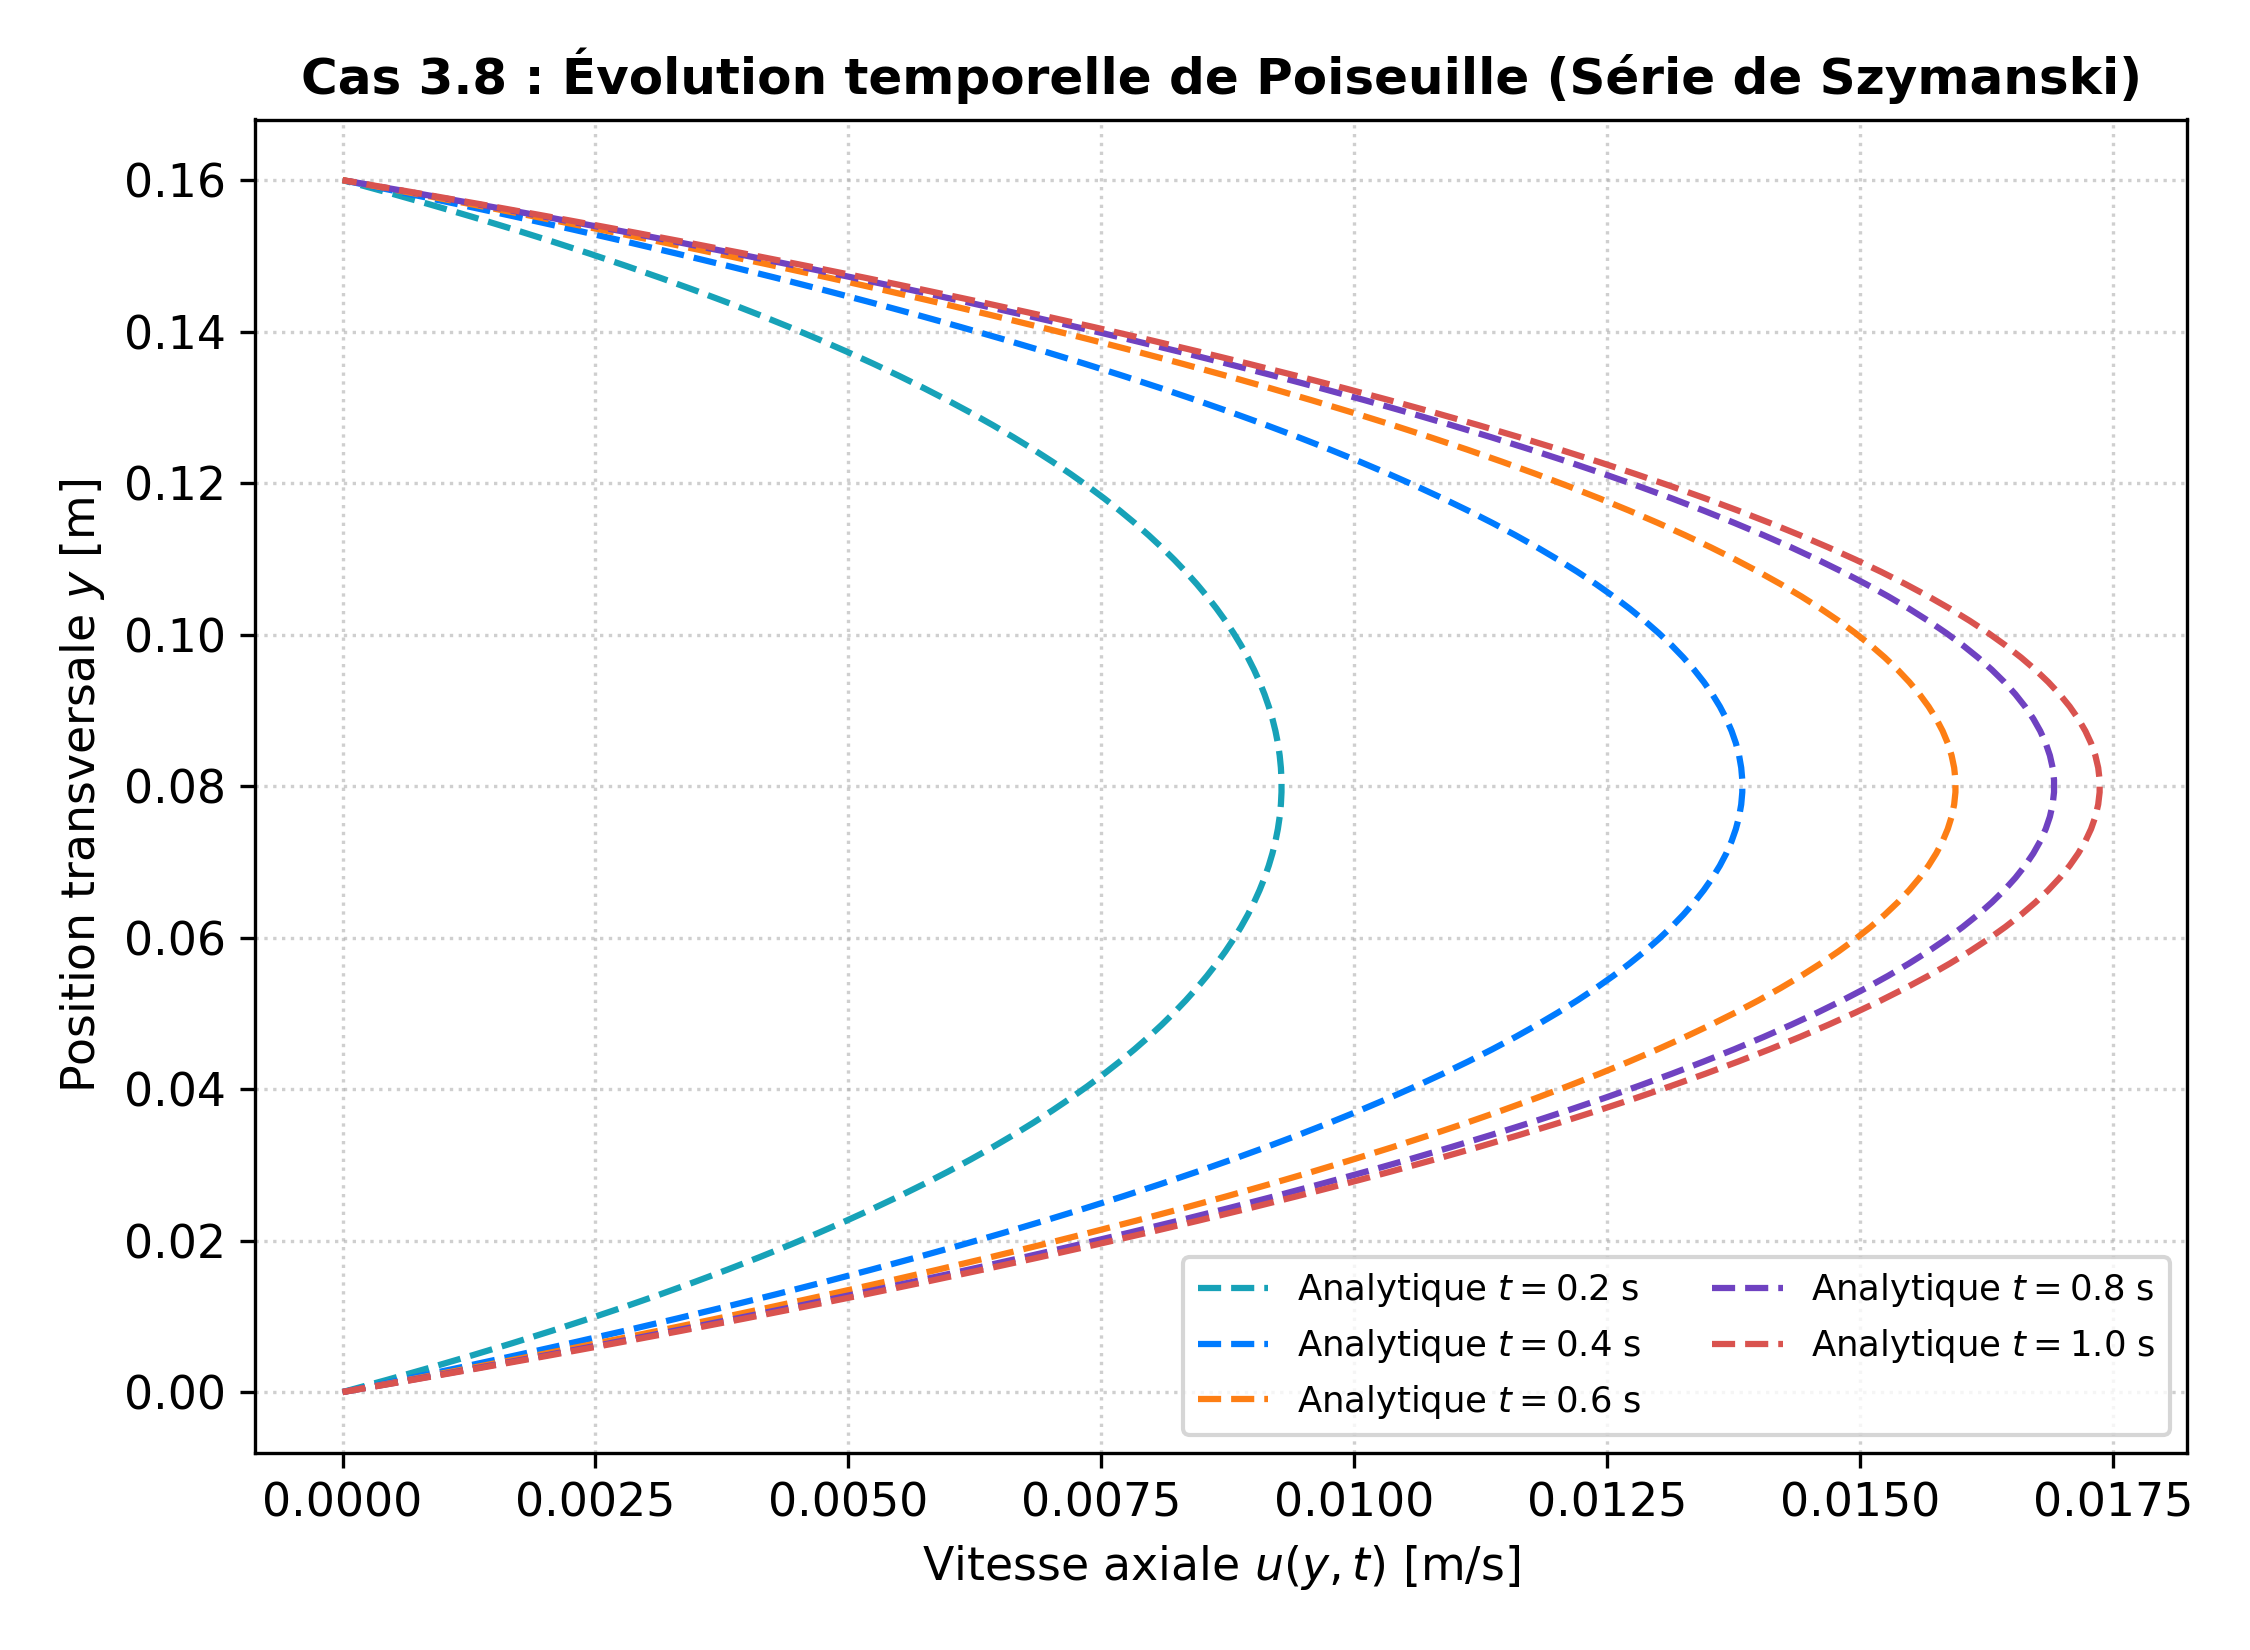
\includegraphics[keepaspectratio,alt={Szymanski Cas
3.8}]{docs/figures/fig_cas3_8_szymanski_unsteady.png}} &
\pandocbounded{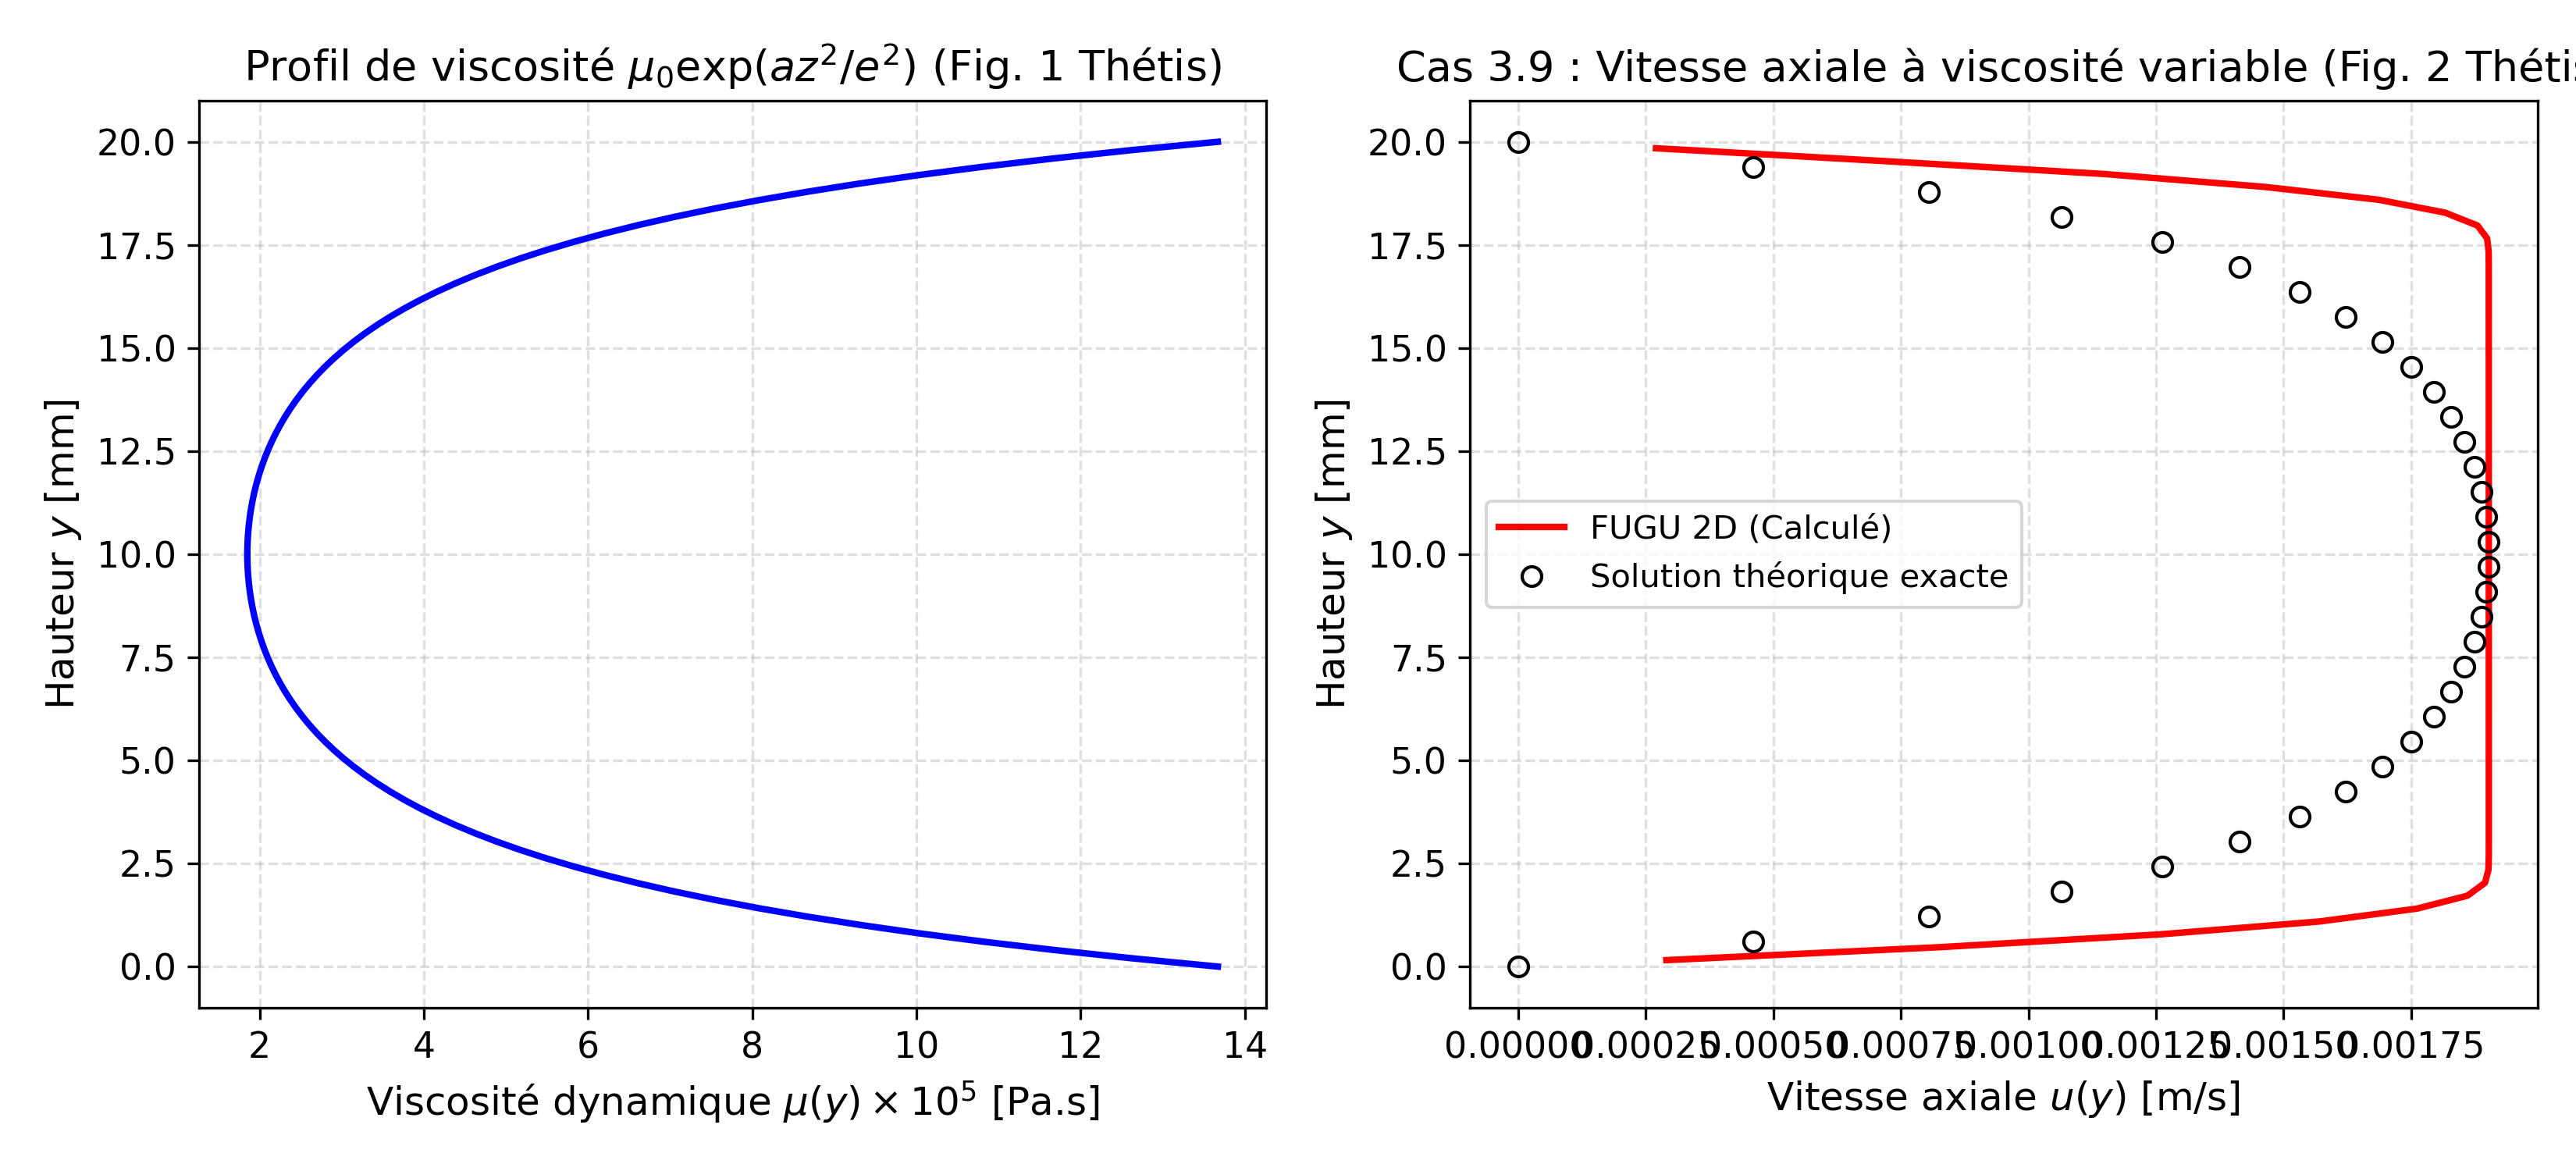
\includegraphics[keepaspectratio,alt={Viscosité Variable
Cas 3.9}]{docs/figures/fig_cas3_9_variable_viscosity.png}} \\
\emph{Profils transitoires aux temps
\(t = 0.2, 0.4, 0.6, 0.8, 1.0\text{ s}\)} & \emph{Superposition
analytique parfaite du profil \(u(y)\)
(\(u_{\max}=0.3436\text{ m/s}\))} \\
\end{longtable}
}

{\def\LTcaptype{none} % do not increment counter
\begin{longtable}[]{@{}
  >{\centering\arraybackslash}p{(\linewidth - 2\tabcolsep) * \real{0.5000}}
  >{\centering\arraybackslash}p{(\linewidth - 2\tabcolsep) * \real{0.5000}}@{}}
\toprule\noalign{}
\begin{minipage}[b]{\linewidth}\centering
Cas 4.1 : Marche Descendante d'Armaly (\(Re=100\))
\end{minipage} & \begin{minipage}[b]{\linewidth}\centering
Cas 4.5 : Lignes de Courant Cavité (\(Re=1000\))
\end{minipage} \\
\midrule\noalign{}
\endhead
\bottomrule\noalign{}
\endlastfoot
\pandocbounded{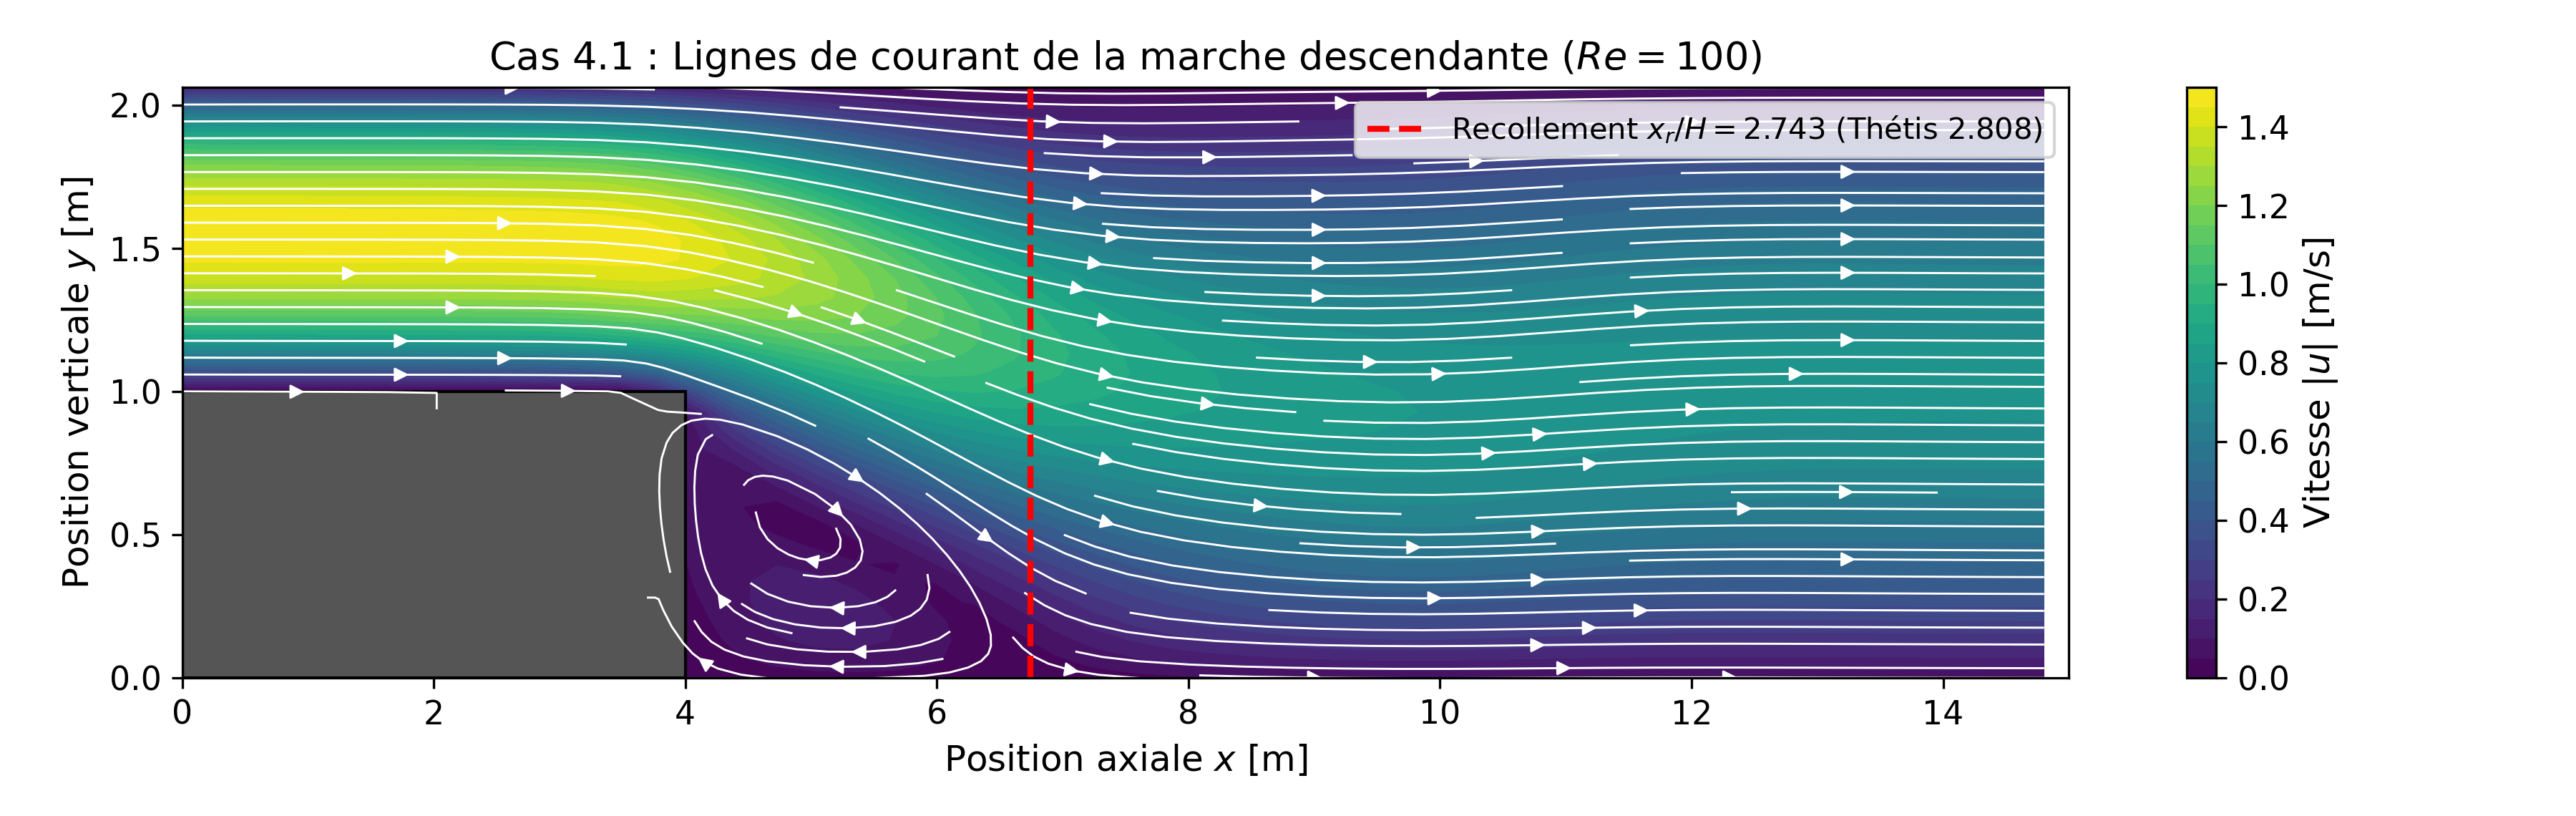
\includegraphics[keepaspectratio,alt={Marche Cas
4.1}]{docs/figures/fig_cas4_1_step_recirculation.png}} &
\pandocbounded{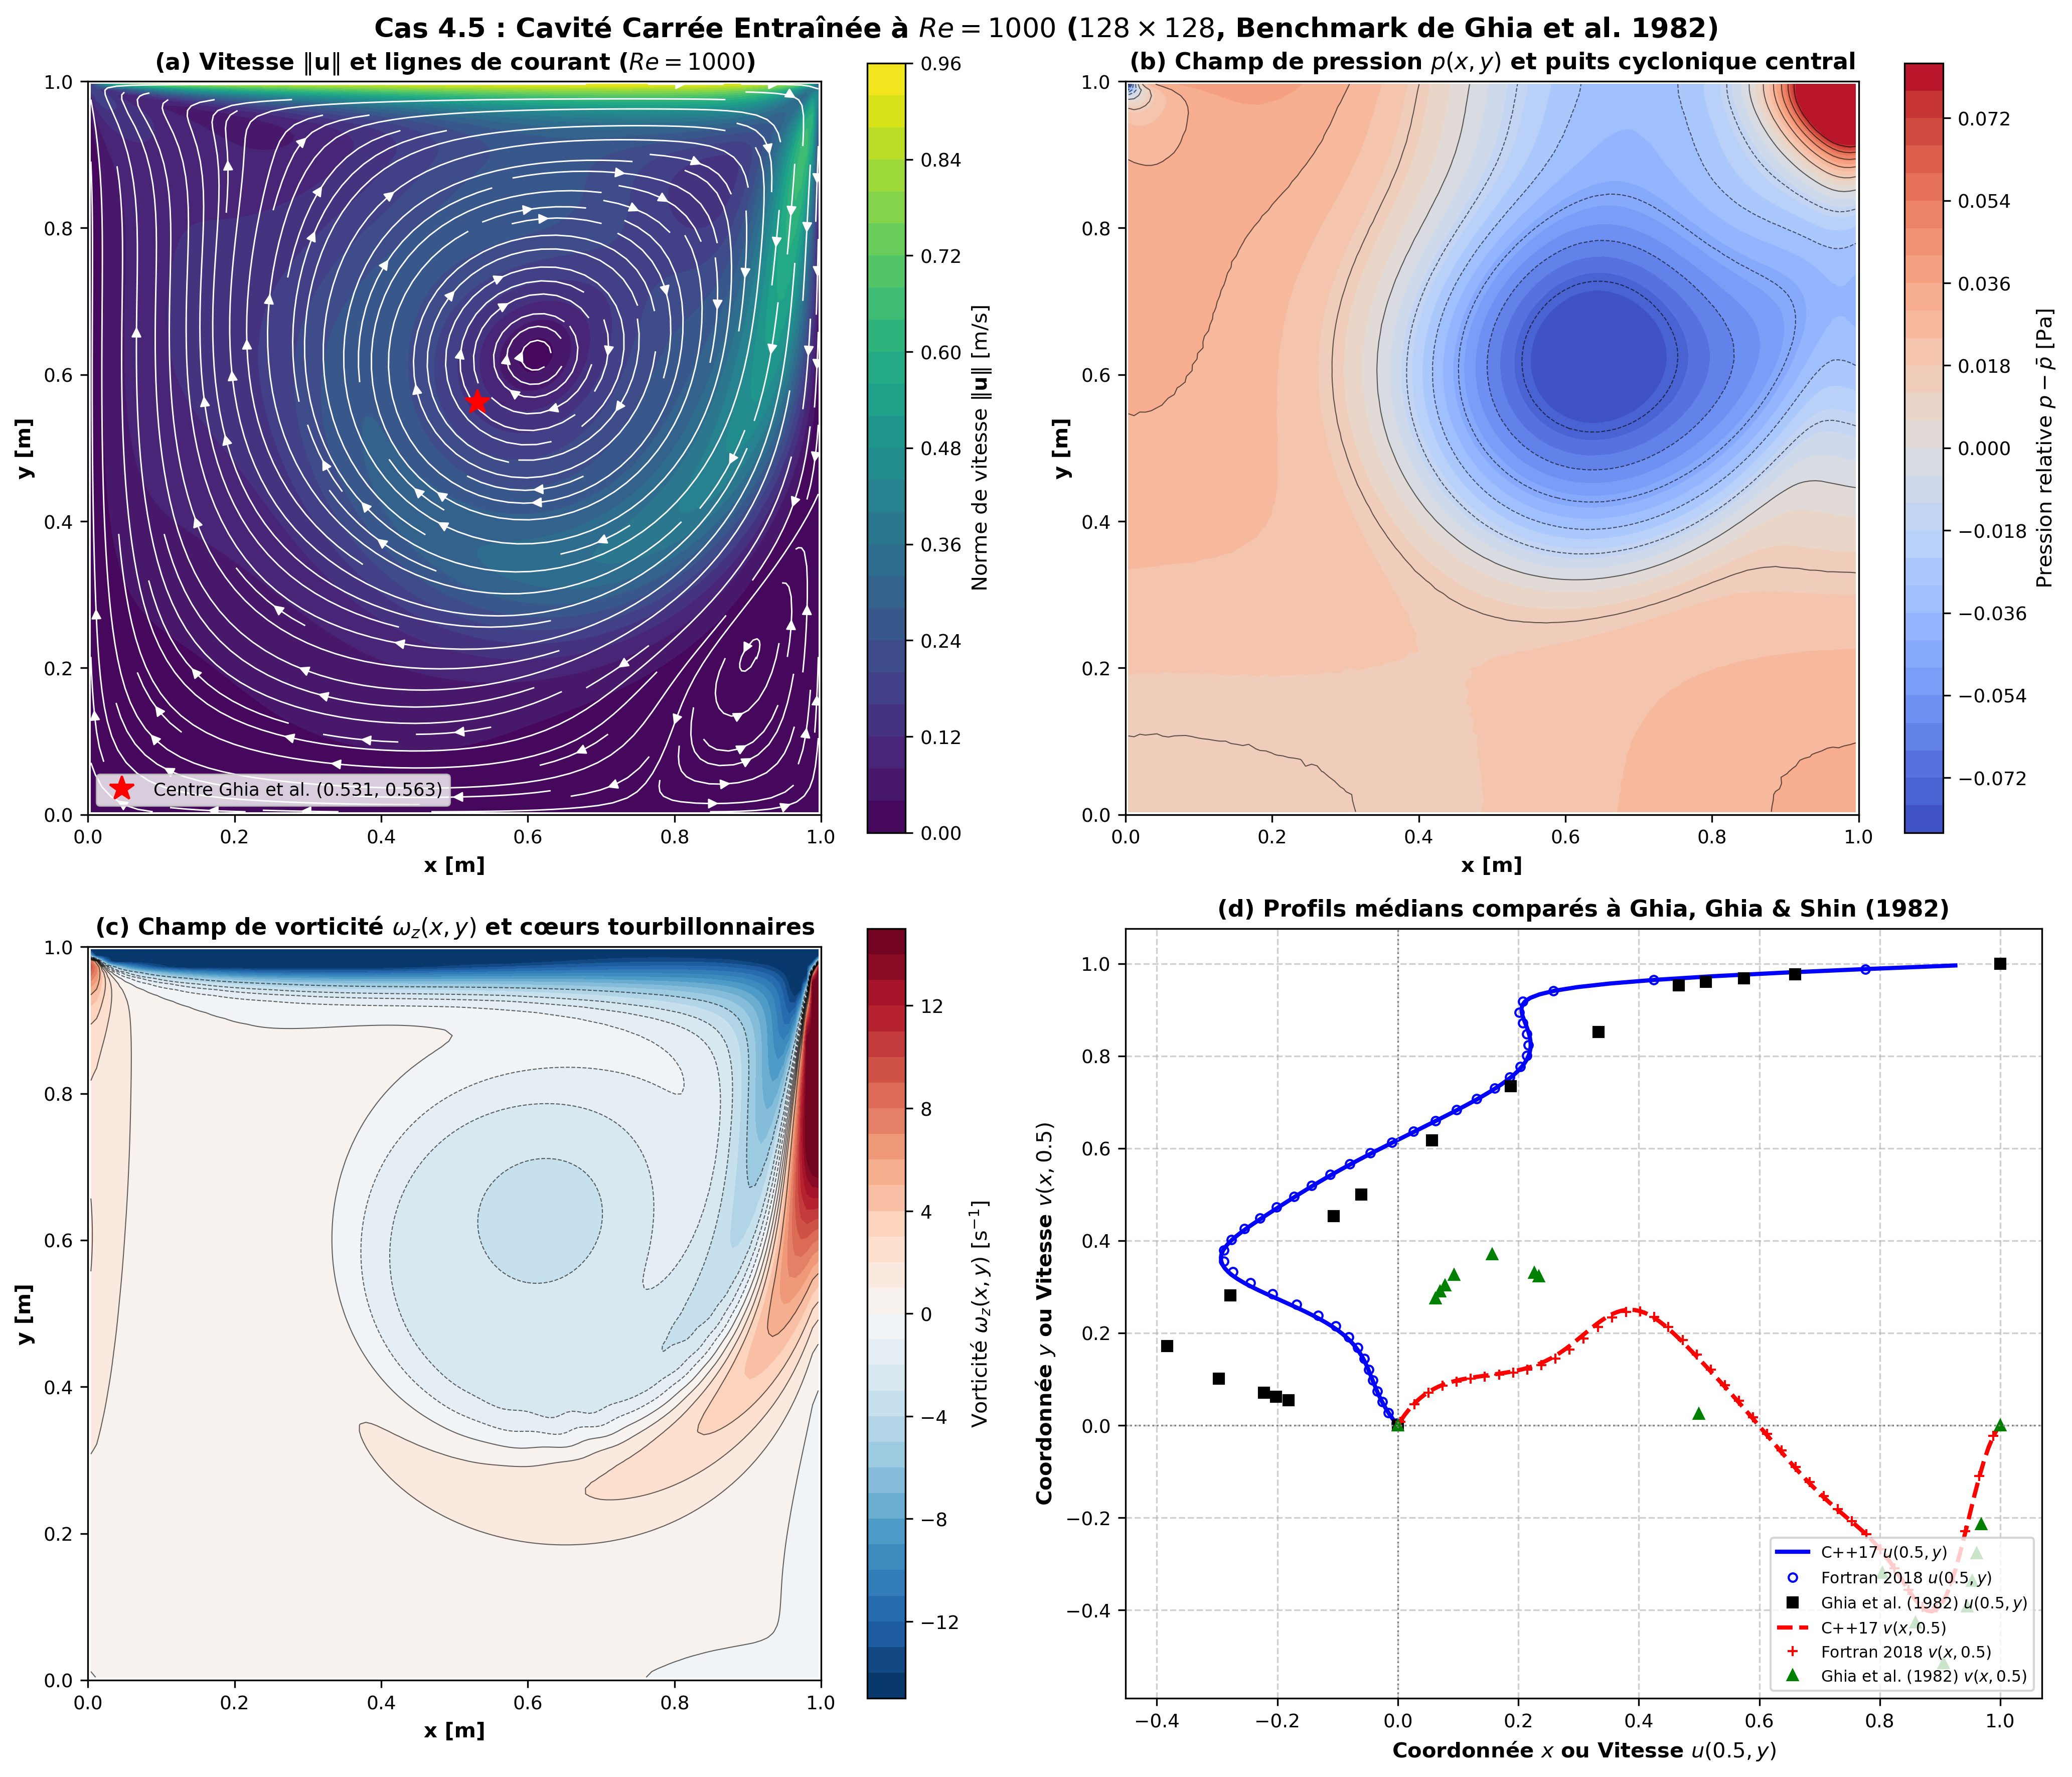
\includegraphics[keepaspectratio,alt={Cavité Cas
4.5}]{docs/figures/fig_cas4_5_cavity_streamlines.png}} \\
\emph{Zone de recirculation primaire avec recollement à
\(x_r/H = 2.719\)} & \emph{Vortex central principal et tourbillons
secondaires de coin} \\
\end{longtable}
}

{\def\LTcaptype{none} % do not increment counter
\begin{longtable}[]{@{}
  >{\centering\arraybackslash}p{(\linewidth - 2\tabcolsep) * \real{0.5000}}
  >{\centering\arraybackslash}p{(\linewidth - 2\tabcolsep) * \real{0.5000}}@{}}
\toprule\noalign{}
\begin{minipage}[b]{\linewidth}\centering
Cas 6.1 : Convection Naturelle (\(Ra=10^4\))
\end{minipage} & \begin{minipage}[b]{\linewidth}\centering
Cas 7.4 : Saut de Pression de Laplace (Goutte)
\end{minipage} \\
\midrule\noalign{}
\endhead
\bottomrule\noalign{}
\endlastfoot
\pandocbounded{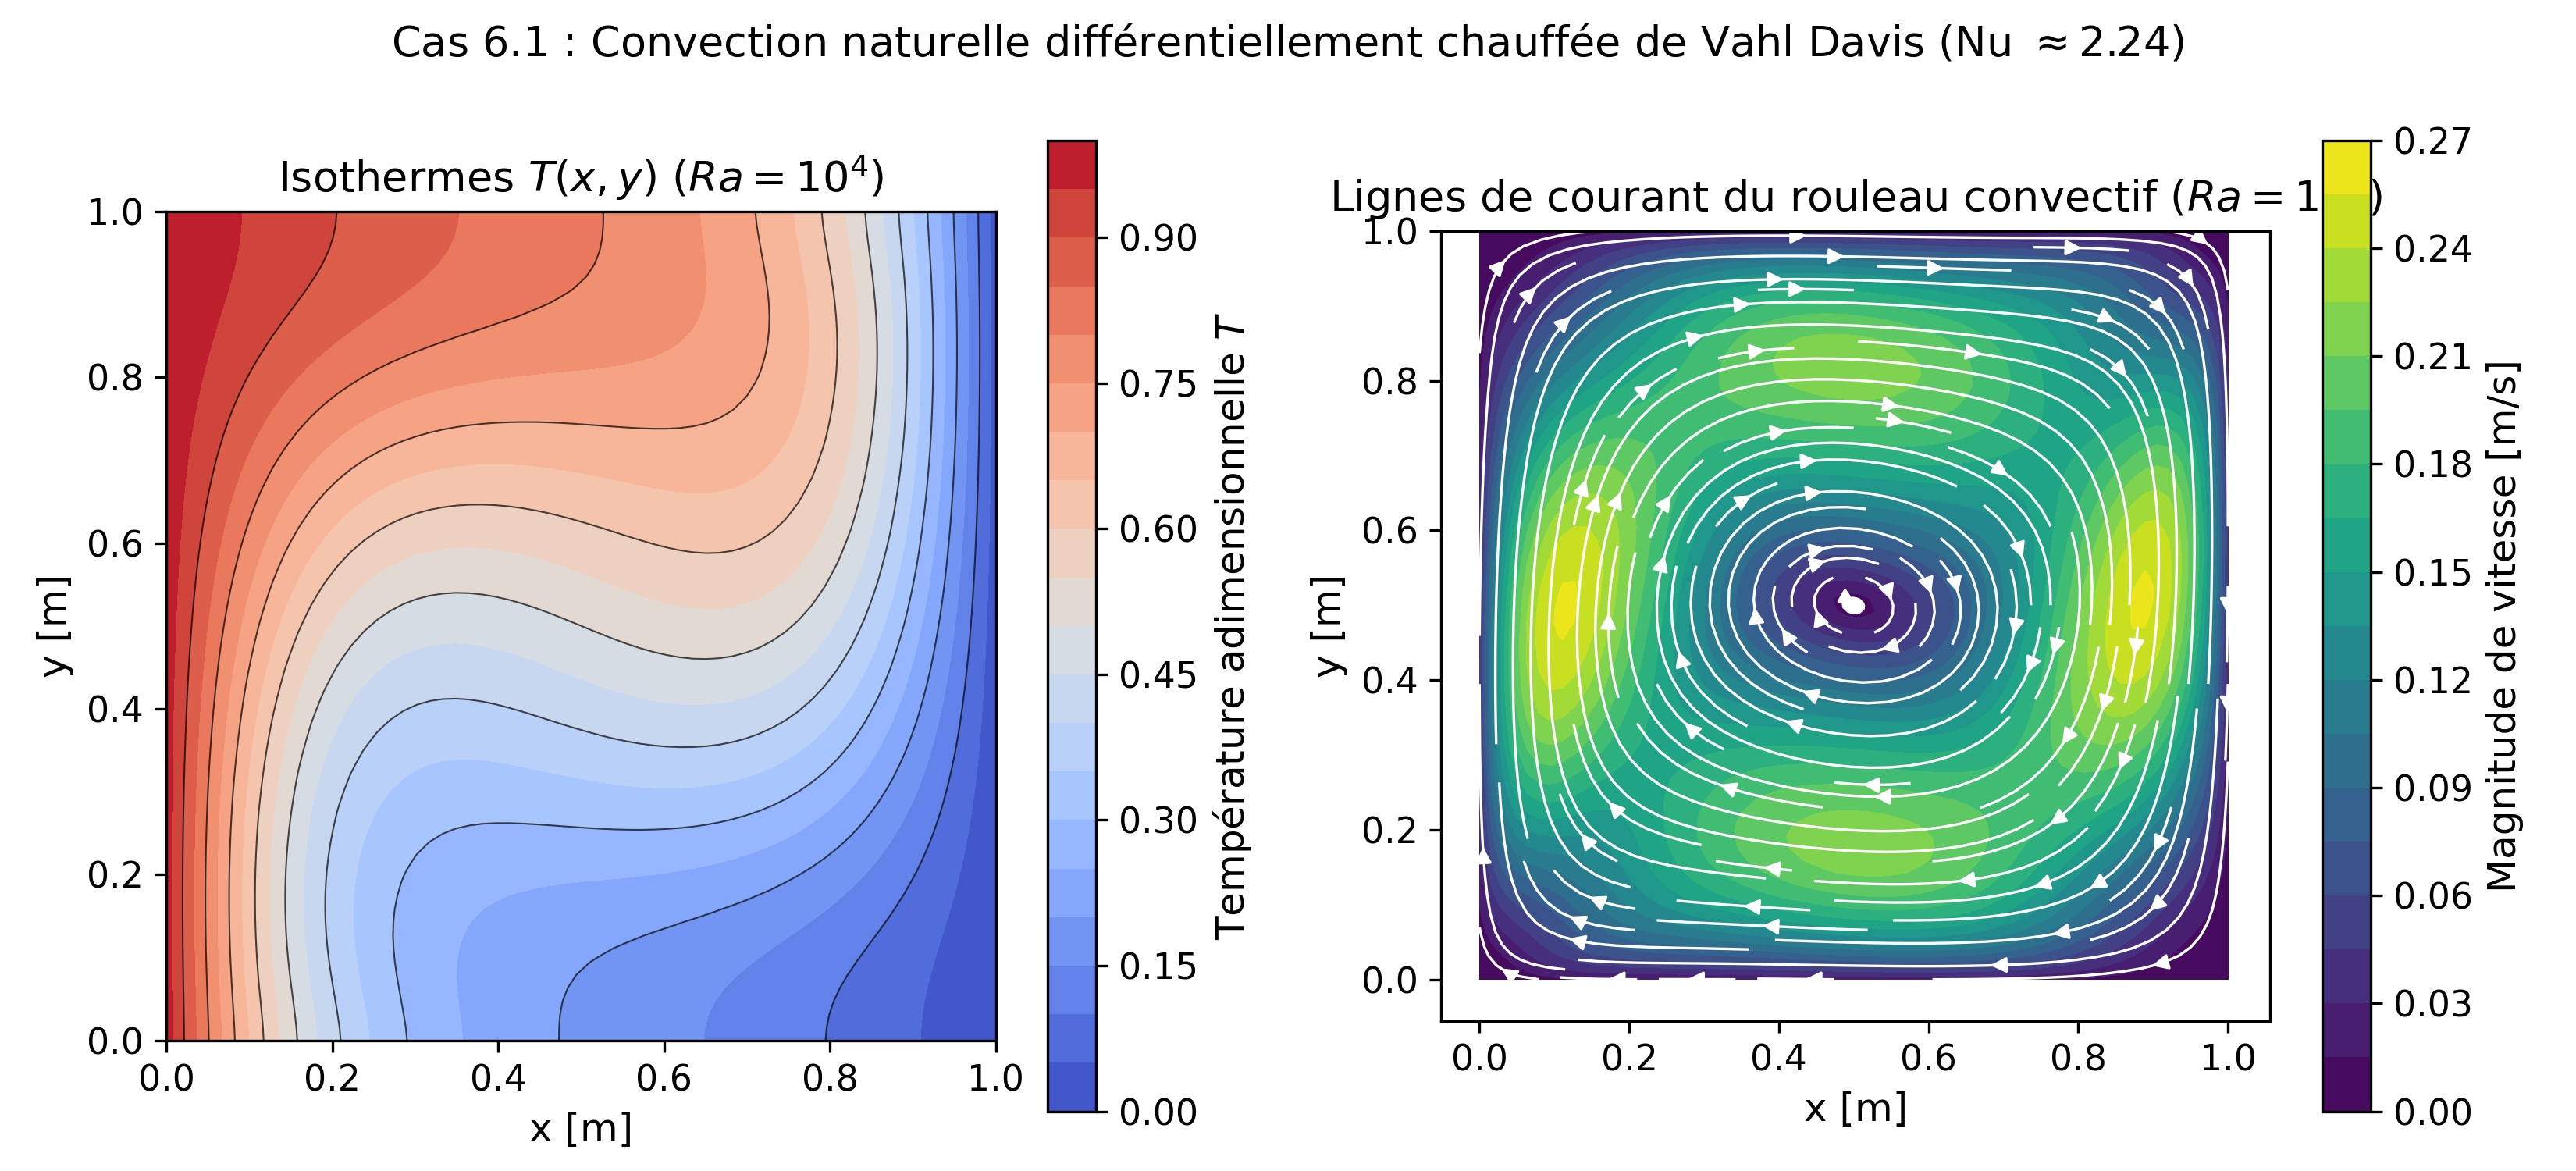
\includegraphics[keepaspectratio,alt={Convection Cas
6.1}]{docs/figures/fig_cas6_1_natural_convection.png}} &
\pandocbounded{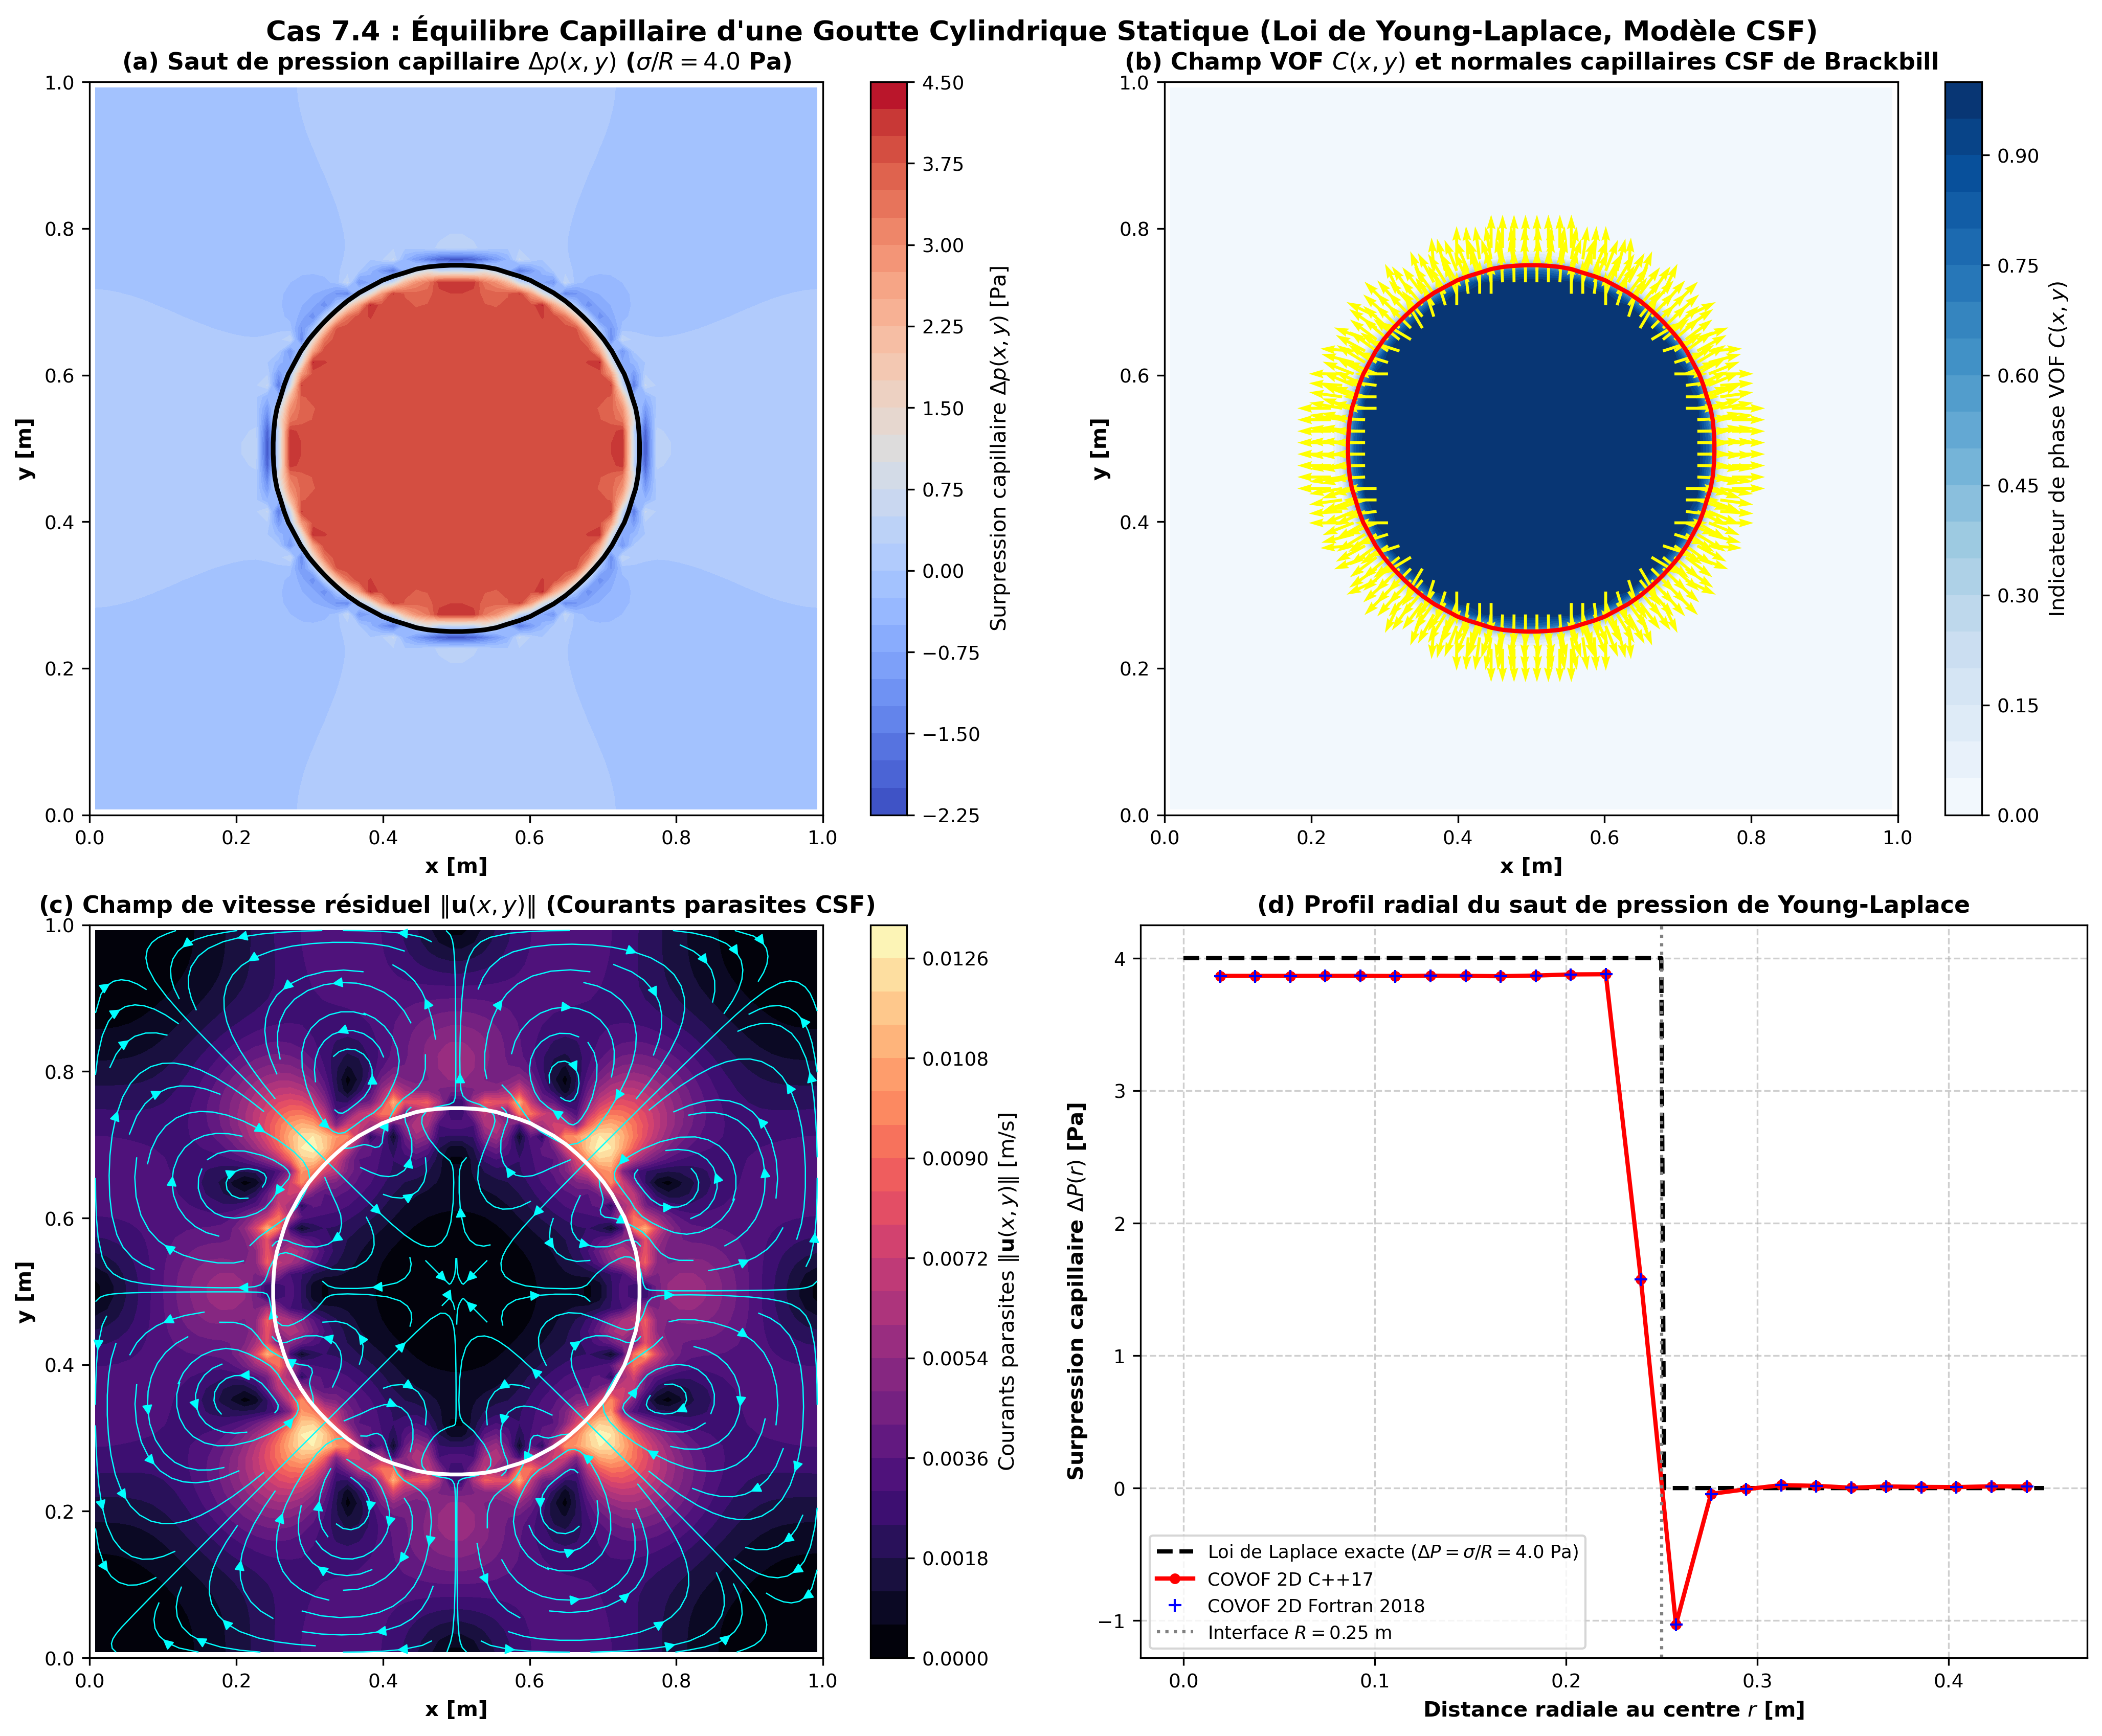
\includegraphics[keepaspectratio,alt={Goutte Laplace Cas
7.4}]{docs/figures/fig_cas7_4_laplace_droplet.png}} \\
\emph{Rouleau de recirculation thermique et isothermes
(\(\overline{Nu} = 2.40\))} & \emph{Profil radial de pression
\(\Delta P = \sigma / R = 4.0\text{ Pa}\)} \\
\end{longtable}
}

\begin{center}\rule{0.5\linewidth}{0.5pt}\end{center}

\subsection{🛠 Prérequis et
Dépendances}\label{pruxe9requis-et-duxe9pendances}

\subsubsection{Environnement Logiciel}\label{environnement-logiciel}

\begin{itemize}
\tightlist
\item
  \textbf{Compilateur Fortran} : GFortran 9+ (supportant Fortran 2018)
  ou Intel oneAPI \texttt{ifx} / \texttt{ifort}.
\item
  \textbf{Bibliothèque MPI} : OpenMPI 4.0+ ou MPICH 3.3+ compilée avec
  les liaisons Fortran (\texttt{mpifort}).
\item
  \textbf{Système de Build} : CMake 3.18+ (ou compilation directe via
  \texttt{mpifort}).
\item
  \textbf{Environnement Python (Optionnel pour post-traitement)} :
  Python 3.8+ (\texttt{numpy}, \texttt{matplotlib}, \texttt{pandas}).
\item
  \textbf{Visualisation 2D/3D} :
  \href{https://www.paraview.org/}{ParaView} (fichiers maîtres
  multi-processus \texttt{.pvtr}).
\end{itemize}

\subsubsection{Installation des
Prérequis}\label{installation-des-pruxe9requis}

\begin{itemize}
\item
  \textbf{macOS (Homebrew)} :

\begin{Shaded}
\begin{Highlighting}[]
\ExtensionTok{brew}\NormalTok{ install cmake open{-}mpi gcc}
\end{Highlighting}
\end{Shaded}
\item
  \textbf{Ubuntu / Debian} :

\begin{Shaded}
\begin{Highlighting}[]
\FunctionTok{sudo}\NormalTok{ apt{-}get update}
\FunctionTok{sudo}\NormalTok{ apt{-}get install }\AttributeTok{{-}y}\NormalTok{ gfortran cmake libopenmpi{-}dev openmpi{-}bin}
\end{Highlighting}
\end{Shaded}
\end{itemize}

\begin{center}\rule{0.5\linewidth}{0.5pt}\end{center}

\subsection{📦 Compilation et Installation
Rapide}\label{compilation-et-installation-rapide}

\subsubsection{Option A : Via CMake
(Recommandé)}\label{option-a-via-cmake-recommanduxe9}

\begin{Shaded}
\begin{Highlighting}[]
\CommentTok{\# 1. Cloner le dépôt}
\FunctionTok{git}\NormalTok{ clone https://github.com/EL{-}I{-}Thiam/COVOF\_2D{-}FORTRAN.git}
\BuiltInTok{cd}\NormalTok{ COVOF\_2D{-}FORTRAN}

\CommentTok{\# 2. Configurer et compiler}
\FunctionTok{cmake} \AttributeTok{{-}B}\NormalTok{ build }\AttributeTok{{-}DCMAKE\_BUILD\_TYPE}\OperatorTok{=}\NormalTok{Release}
\FunctionTok{cmake} \AttributeTok{{-}{-}build}\NormalTok{ build }\AttributeTok{{-}j4}

\CommentTok{\# 3. Vérifier le binaire produit}
\FunctionTok{ls} \AttributeTok{{-}lh}\NormalTok{ bin/covof2d\_fortran}
\end{Highlighting}
\end{Shaded}

\subsubsection{Option B : Compilation Directe
Standalone}\label{option-b-compilation-directe-standalone}

Si CMake n'est pas disponible, vous pouvez compiler directement
l'ensemble des modules ordonnés en une seule ligne de commande :

\begin{Shaded}
\begin{Highlighting}[]
\ExtensionTok{mpifort} \AttributeTok{{-}O3} \AttributeTok{{-}march}\OperatorTok{=}\NormalTok{native }\DataTypeTok{\textbackslash{}}
\NormalTok{  src/module\_precision.f90 }\DataTypeTok{\textbackslash{}}
\NormalTok{  src/module\_constants.f90 }\DataTypeTok{\textbackslash{}}
\NormalTok{  src/module\_json.f90 }\DataTypeTok{\textbackslash{}}
\NormalTok{  src/module\_config.f90 }\DataTypeTok{\textbackslash{}}
\NormalTok{  src/module\_mesh.f90 }\DataTypeTok{\textbackslash{}}
\NormalTok{  src/module\_fields.f90 }\DataTypeTok{\textbackslash{}}
\NormalTok{  src/module\_mpi\_comm.f90 }\DataTypeTok{\textbackslash{}}
\NormalTok{  src/module\_interface\_vof.f90 }\DataTypeTok{\textbackslash{}}
\NormalTok{  src/module\_navier\_stokes.f90 }\DataTypeTok{\textbackslash{}}
\NormalTok{  src/module\_linear\_solvers.f90 }\DataTypeTok{\textbackslash{}}
\NormalTok{  src/module\_vtk\_writer.f90 }\DataTypeTok{\textbackslash{}}
\NormalTok{  src/module\_simulation.f90 }\DataTypeTok{\textbackslash{}}
\NormalTok{  src/covof2d\_main.f90 }\DataTypeTok{\textbackslash{}}
  \AttributeTok{{-}o}\NormalTok{ bin/covof2d\_fortran}
\end{Highlighting}
\end{Shaded}

\begin{center}\rule{0.5\linewidth}{0.5pt}\end{center}

\subsection{⚡ Guide d'Exécution
Rapide}\label{guide-dexuxe9cution-rapide}

\subsubsection{1. Lancer une simulation
individuelle}\label{lancer-une-simulation-individuelle}

Pour exécuter un cas test avec \(N\) processus MPI :

\begin{Shaded}
\begin{Highlighting}[]
\CommentTok{\# Cavité entraînée Re=1000 sur 4 processus}
\ExtensionTok{mpirun} \AttributeTok{{-}np}\NormalTok{ 4 bin/covof2d\_fortran cases/cavity\_re1000.json}

\CommentTok{\# Écoulement autour d\textquotesingle{}un cylindre Re=20 sur 2 processus}
\ExtensionTok{mpirun} \AttributeTok{{-}np}\NormalTok{ 2 bin/covof2d\_fortran cases/obstacle\_cylinder\_re20.json}

\CommentTok{\# Rupture de barrage VOF sur 4 processus}
\ExtensionTok{mpirun} \AttributeTok{{-}np}\NormalTok{ 4 bin/covof2d\_fortran cases/dam\_break.json}
\end{Highlighting}
\end{Shaded}

\subsubsection{2. Exécuter l'ensemble de la suite de validation (13
cas)}\label{exuxe9cuter-lensemble-de-la-suite-de-validation-13-cas}

Le script automatisé
\href{scripts/run_all_benchmarks.sh}{\texttt{scripts/run\_all\_benchmarks.sh}}
compile, exécute tous les cas de calcul en parallèle, analyse les
résultats et affiche le rapport de validation :

\begin{Shaded}
\begin{Highlighting}[]
\ExtensionTok{./scripts/run\_all\_benchmarks.sh}\NormalTok{ 2}
\end{Highlighting}
\end{Shaded}

\subsubsection{3. Vérifier les métriques et générer les
figures}\label{vuxe9rifier-les-muxe9triques-et-guxe9nuxe9rer-les-figures}

\begin{Shaded}
\begin{Highlighting}[]
\CommentTok{\# Vérification des erreurs L1 / Linf et génération du rapport Markdown / CSV}
\ExtensionTok{python3}\NormalTok{ scripts/verify\_cases.py}

\CommentTok{\# Génération des 14 figures comparatives haute définition}
\ExtensionTok{python3}\NormalTok{ scripts/generate\_validation\_figures.py}
\end{Highlighting}
\end{Shaded}

\begin{center}\rule{0.5\linewidth}{0.5pt}\end{center}

\subsection{📁 Structure du Dépôt}\label{structure-du-duxe9puxf4t}

\begin{verbatim}
covof2d_fortran/
├── CMakeLists.txt                # Configuration CMake Fortran 2018 / MPI
├── TUTORIAL.md                   # Tutoriel pas à pas complet pour COVOF 2D Fortran
├── validation_summary.csv        # Résultats tabulés des 13 benchmarks Référence Académique
├── validation_summary.md         # Synthèse Markdown des métriques CFD
├── bin/                          # Exécutable binaire covof2d_fortran
├── src/                          # 12 modules Fortran 2018 et programme principal
│   ├── module_precision.f90      # Précision double standardisée (dp = real64)
│   ├── module_constants.f90      # Constantes physiques et numériques fondamentales
│   ├── module_json.f90           # Parseur JSON natif Fortran pour fichiers de cas
│   ├── module_config.f90         # Structures de configuration et validation
│   ├── module_mesh.f90           # Décomposition 2D et métrique cartésienne
│   ├── module_fields.f90         # Champs de vitesse (MAC), pression, température, VOF
│   ├── module_mpi_comm.f90       # Gestion des halos fantômes et communications non-bloquantes
│   ├── module_interface_vof.f90  # Transport VOF-TVD Superbee et modèle CSF
│   ├── module_navier_stokes.f90  # Discrétisation spatiale complète, Uzawa et Boussinesq
│   ├── module_linear_solvers.f90 # Solveurs BiCGSTAB2, PCG, GMRES Matrix-Free
│   ├── module_vtk_writer.f90     # Exporteur rectilinéaire multi-blocs .pvtr/.vtr
│   ├── module_simulation.f90     # Boucle temporelle et orchestration
│   └── covof2d_main.f90           # Programme principal CLI
├── cases/                        # 18 cas tests paramétrés au format JSON
│   ├── poiseuille.json           # Cas 3.7 : Poiseuille plan stationnaire
│   ├── poiseuille_unsteady.json  # Cas 3.8 : Poiseuille transitoire de Szymanski
│   ├── poiseuille_variable_viscosity.json # Cas 3.9 : Viscosité variable exponentielle
│   ├── vortex_shear_advection.json        # Cas 3.19 : Vortex avec cisaillement
│   ├── backward_facing_step.json          # Cas 4.1 : Marche descendante d'Armaly
│   ├── obstacle_cylinder_re20.json        # Cas 4.4 : Sillage de cylindre Re=20
│   ├── cavity_re1000.json        # Cas 4.5 : Cavité entraînée Re=1000
│   ├── cavity_l_shaped.json      # Cas 4.7 : Cavité en forme de L
│   ├── natural_convection_ra1e4.json # Cas 6.1 : Convection de Vahl Davis
│   ├── dam_break.json            # Cas 7.1 : Rupture de barrage diphasique
│   ├── static_droplet.json       # Cas 7.4 : Goutte statique et loi de Laplace
│   └── rising_bubble.json        # Cas 7.5 : Bulle ascendante (Hysing)
├── docs/                         # Documentation technique complète (>45 pages)
│   ├── INDEX.md                  # Sommaire général de la documentation
│   ├── USER_GUIDE.md             # Manuel de référence utilisateur
│   ├── DEVELOPER_GUIDE.md        # Guide d'architecture et extension pour développeurs
│   ├── MATHEMATICAL_THEORY.md    # Dérivations théoriques et discrétisations
│   ├── VALIDATION_GUIDE.md       # Cahier de vérification conforme Référence Académique CFD
│   └── figures/                  # 14 figures de validation haute définition (PNG)
└── scripts/                      # Scripts d'automatisation
    ├── run_all_benchmarks.sh     # Script bash de lancement de tous les calculs
    ├── verify_cases.py           # Analyse de convergence et validation automatique
    └── generate_validation_figures.py # Générateur de graphiques comparatifs
\end{verbatim}

\begin{center}\rule{0.5\linewidth}{0.5pt}\end{center}

\subsection{📖 Documentation et Tutoriels
Détaillés}\label{documentation-et-tutoriels-duxe9tailluxe9s}

\begin{itemize}
\tightlist
\item
  \href{TUTORIAL.md}{\textbf{Tutoriel Pratique Exhaustif
  (\texttt{TUTORIAL.md})}} : guide d'apprentissage étape par étape
  adapté à Fortran 2018 pour paramétrer, simuler et post-traiter des
  écoulements CFD.
\item
  \href{docs/USER_GUIDE.md}{\textbf{Manuel Utilisateur
  (\texttt{docs/USER\_GUIDE.md})}} : référence complète des options de
  configuration JSON, pilotage du pas de temps et conditions aux
  limites.
\item
  \href{docs/DEVELOPER_GUIDE.md}{\textbf{Guide Développeur
  (\texttt{docs/DEVELOPER\_GUIDE.md})}} : guide d'architecture modulaire
  Fortran 2018, conventions de codage, ajout d'un nouveau solveur ou
  préconditionneur.
\item
  \href{docs/MATHEMATICAL_THEORY.md}{\textbf{Documentation Théorique
  (\texttt{docs/MATHEMATICAL\_THEORY.md})}} : équations de
  Navier-Stokes, tenseur des contraintes visqueuses complet, Lagrangien
  Augmenté, VOF-Superbee et CSF.
\item
  \href{docs/VALIDATION_GUIDE.md}{\textbf{Cahier de Validation
  (\texttt{docs/VALIDATION\_GUIDE.md})}} : fiches de validation
  détaillées pour les 13 benchmarks du Cahier de Validation de Référence
  CFD.
\end{itemize}

\begin{center}\rule{0.5\linewidth}{0.5pt}\end{center}

\subsection{👥 Auteurs et Licence}\label{auteurs-et-licence}

\begin{itemize}
\tightlist
\item
  \textbf{Auteur \& Développeur} : Elhadji Ibrahima Thiam
\item
  \textbf{Laboratoire d'Inspiration} : I2M / Laboratoire TREFLE
  (Bordeaux) --- Projet Référence Académique
\item
  \textbf{Licence} : Ce projet est distribué sous licence open-source
  MIT.
\end{itemize}

\end{document}
